\documentclass{article}
\usepackage{amsmath}
\usepackage{graphicx}
\usepackage{multicol}
\usepackage[margin=1in]{geometry}
\usepackage{xcolor}
\usepackage{amssymb}
\begin{document}
% Header layout
\begin{minipage}{0.6\textwidth}
    
\includegraphics[height=1.8cm]{img3.png}
\end{minipage}
\hfill
\begin{minipage}{0.35\textwidth}
\raggedleft
\textbf{Name:} K.Saisusmitha \\
\textbf{Batch:} COMETFWC018 \\
\textbf{Date:} 4 June 2025
\end{minipage}

\begin{center}
    {\color{cyan} \LARGE \textbf{GATE QUESTION}}\\
    {\color{cyan} \Large \textbf{ECE 2010 Q39}}
\end{center}
\vspace{1em}
\noindent\textbf{\color{cyan} Q39.} The Boolean function realized by the logic circuit shown is:

\vspace{1em}

% Include the image (make sure this file exists in your directory)
\begin{center}
    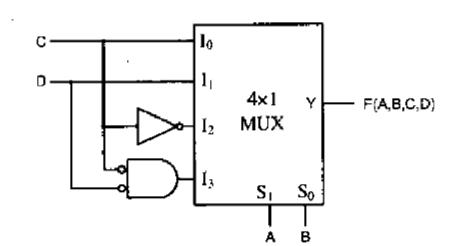
\includegraphics[width=0.7\textwidth]{esp 32.png} 
\end{center}

\vspace{1em}

\noindent\textbf{Options:}

\vspace{0.5em}
\begin{multicols}{2}
\begin{itemize}
    \item[(A)] \(F = \Sigma m(0,1,3,5,9,10,14)\)
    \item[(B)] \(F = \Sigma m(2,3,5,7,8,12,13)\)
    \item[(C)] \(F = \Sigma m(1,2,4,5,11,14,15)\)
    \item[(D)] \(F = \Sigma m(2,3,5,7,8,9,12)\)
\end{itemize}
\end{multicols}


\section*{\color{cyan} Solution :}

Output of the MUX can be written as:
\[
F = I_0 \overline{S_0} \, \overline{S_1} + I_1 S_0 \, \overline{S_1} + I_2 \overline{S_0} S_1 + I_3 S_0 S_1
\]

Here, \[
I_0 = C, \quad I_1 = D, \quad I_2 = \overline{C}, \quad I_3 = CD
\]
and \[
S_0 = A, \quad S_1 = B
\]

So,
\[
F = C \, \overline{A} \, \overline{B} + D A \, \overline{B} + \overline{C} \, \overline{A} B + CD A B
\]

Writing all SOP terms:
\[
F = \overline{A} \, \overline{B} \, C \, \overline{D} 
+ \overline{A} \, \overline{B} \, C D 
+ \overline{A} B \, \overline{C} \, \overline{D} 
+ \overline{A} B \, \overline{C} D 
+ A \, \overline{B} \, D \, \overline{C} 
+ A \, \overline{B} \, D C 
+ A B C D
\]

\[
F = \Sigma m(2, 3, 5, 7, 8, 9, 12)
\]

Hence, (D) is the correct option.

\end{document}
